\documentclass[12pt]{article}
\usepackage[utf8]{inputenc}
\usepackage[draft]{moodle}
\usepackage{graphicx}

% Commands for jinja2 templating
% Instead of empty braces (i.e. no command effect), here we make the variable uppercase red
% to emphasize in the template those variables to be replaced. Once rendered, this formatting
% has not effect as jinja replaces the \VAR{variable} entirely.
\usepackage{xcolor}
\newcommand*{\VAR}[1]{\textcolor{red}{\textbf{#1}}}

%\moodle@draftmodetrue
%\moodle@draftmodefalse

\begin{document}
\begin{quiz}{Quiz No. \VAR{id}}
	
\begin{numerical}[points=2]{Basic addition}
	What is \VAR{A} + \VAR{B}?	
	\item \VAR{C}
\end{numerical}

\begin{shortanswer}[case sensitive=true]{Bridge Type}
	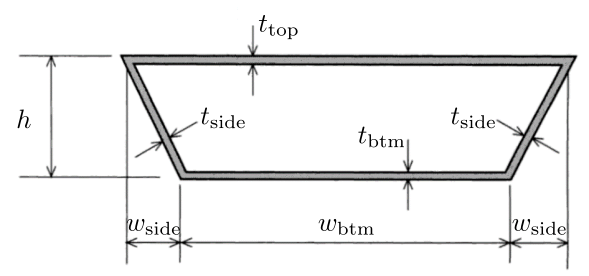
\includegraphics[width=8cm]{./media/image1}
	
	This is a
	\item* \VAR{text}
	\item[fraction=0, feedback={No, silly!}] picture
	\item[fraction=0] bridge
\end{shortanswer}
	
\begin{cloze}[feedback=Please hover to see specific feedback]{Circles} 
	
	A circle has radius \VAR{radius}, what is its area?
	
	\begin{numerical}[points=1,penalty=0]
		\item[feedback = {Well done!},tolerance = \VAR{areatol}] \VAR{area}
		\item[fraction = 0,feedback = {Note the units.}] * % All other incorrect answers
	\end{numerical}

	A circle has area \VAR{area2}, what is its radius?

	\begin{numerical}[points=1,penalty=0]
		\item[feedback = {Well done!},tolerance = \VAR{radius2tol}] \VAR{radius2}
		\item[fraction = 0,feedback = {Note the units.}] * % All other incorrect answers
	\end{numerical}	
	
	Provide your answers to 3 significant figures, in the units shown, and using engineering notation as necessary.
	
\end{cloze}

\begin{multi}[points=3]{A first derivative}
What is the first derivative of $x^3$?
\item $\frac{1}{4} x^4+C$
\item* $3x^2$
\item \VAR{D}
\end{multi}

\end{quiz}

\end{document}
